\RequirePackage{fix-cm}
\RequirePackage[hyphens]{url}
\RequirePackage[final]{graphicx} % need to show figures in draft mode
\documentclass[rmp,nofootinbib,superscriptaddress,12pt,tightenlines,notitlepage]{revtex4-1}

\setlength\topmargin{0pt}
\addtolength\topmargin{-\headheight}
\addtolength\topmargin{-\headsep}
\setlength\oddsidemargin{0pt}
\setlength\textwidth{\paperwidth}
\addtolength\textwidth{-2in}
\setlength\textheight{\paperheight}
\addtolength\textheight{-2in}
\usepackage{layout}

% Change to a sans serif font.
\usepackage{sourcesanspro}
\renewcommand*\familydefault{\sfdefault} %% Only if the base font of the document is to be sans serif
\usepackage[T1]{fontenc}
%\usepackage[font=sf,justification=justified]{caption}
\usepackage[font=sf]{floatrow}

% Rework captions to use sans serif font.
\makeatletter
\renewcommand\@make@capt@title[2]{%
 \@ifx@empty\float@link{\@firstofone}{\expandafter\href\expandafter{\float@link}}%
  {\textbf{#1}}\sf\@caption@fignum@sep#2\quad
}%
\makeatother

%\linespread{0.956}
\usepackage{listings} % For code examples
\usepackage[usenames,dvipsnames,svgnames,table]{xcolor}
\usepackage{amsmath}
\usepackage{amssymb}
\usepackage{graphicx}
\usepackage{dcolumn}
\usepackage{boxedminipage}
\usepackage[colorlinks=true,citecolor=blue,linkcolor=blue]{hyperref}
\usepackage[]{microtype}
\usepackage[obeyFinal]{todonotes}
\usepackage{import}
\usepackage{setspace, siunitx, amsmath,amsfonts, adjustbox,booktabs, cleveref}
%\usepackage{caption}
\usepackage{subcaption}
\usepackage{titlesec}
\usepackage{enumitem}
\usepackage[margin=1.0in]{geometry}
\usepackage{etoolbox}
\patchcmd{\section}
  {\centering}
  {\raggedright}
  {}
  {}
\patchcmd{\subsection}
  {\centering}
  {\raggedright}
  {}
  {}

\graphicspath{{/home/bmanubay/Bryces-prelim-exam/report/images/}}

\usepackage{parskip}
\setlength{\parskip}{4pt} % 1ex plus 0.5ex minus 0.2ex}
\setlength{\parindent}{0pt}

\setcitestyle{super}
\setcounter{secnumdepth}{5}

% Units
\DeclareSIUnit\Molar{\textsc{m}}


% Comments
\newcounter{comment}
\newcommand{\comment}[2][]{%
% initials of the author (optional) + note in the margin
\refstepcounter{comment}%
{%
\setstretch{0.7}% spacing
\todo[inline, color={cyan!45},size=\small]{%
\textbf{\footnotesize [\uppercase{#1}\thecomment]:}~#2}%
}}

% Start supplementary sections

\newcommand{\beginsupplement}{%
        \onecolumngrid
        \setcounter{table}{0}
        \renewcommand{\thetable}{S\arabic{table}}%
        \setcounter{figure}{0}
        \renewcommand{\thefigure}{S\arabic{figure}}%
     }

%\graphicspath{{figures/}}
\floatsetup[table]{capposition=top}

\titlespacing\title{4pt}{12pt plus 4pt minus 2pt}{4pt plus 2pt minus 1pt}
\titlespacing\section{0pt}{12pt plus 4pt minus 2pt}{0pt plus 2pt minus 2pt}
\titlespacing\subsection{0pt}{12pt plus 4pt minus 2pt}{0pt plus 2pt minus 2pt}
\titlespacing\subsubsection{0pt}{12pt plus 4pt minus 2pt}{0pt plus 2pt minus 2pt}

\begin{document}

%%%%%%%%%%%%%%%%%%%%%%%%%%%%%%%%%%%%%%%%%%%%%%%%%%%%%%%%%%%%%%%%%%%%%%%%%%%%%%%%
% DOCUMENT
%%%%%%%%%%%%%%%%%%%%%%%%%%%%%%%%%%%%%%%%%%%%%%%%%%%%%%%%%%%%%%%%%%%%%%%%%%%%%%%%

\title{A method for redesigning molecular mechanics force field parameterization by use of a Bayesian statistical framework}
\author{Bryce C. Manubay} 
\email{bryce.manubay@colorado.edu}
\affiliation{University of Colorado - Department of Chemical and Biological Engineering}
% Date
\date{\today}

%%%%%%%%%%%%%%%%%%%%%%%%%%%%%%%%%%%%%%%%%%%%%%%%%%%%%%%%%%%%%%%%%%%%%%%%%%%%%%%%
% ABSTRACT
%%%%%%%%%%%%%%%%%%%%%%%%%%%%%%%%%%%%%%%%%%%%%%%%%%%%%%%%%%%%%%%%%%%%%%%%%%%%%%%%
\maketitle
\section{Objectives}
Molecular dynamics (MD) simulation is fast becoming a more useful tool in many scientific studies. MD simulations are often used in fields However, some limitations remain in the ability of MD force fields to accurately and transferably describe molecular environments. Currently, force fields are parameterized with fixed functional forms with, often, poor physical motivation and require the chemical intuition of experts to manually correct parameters, leading to a more suitable product. Additionally, the creation of a transferable method to update existing force fields based on new experimental data is limited due to lack of understanding and lack of consistency in how the original parameterization was done.

A possible solution to these problems is by recasting the force field parameterization process as a bayesian inference problem. The objective of this paper is introduce a framework for using high quality experimental data in order to automatically generate families of MD force fields consistent with the data used. In this paper I will describe the overall parameterization framework and my roles in the project thus far, first, collecting and curating large amounts of high quality experimental thermochemical data and, currently, investigating use of the Multistate Bennett Acceptance Ratio (MBAR) as a means to improve parameterization throughput by reducing computational expense while making updates to the posterior distribution of parameter sets consistent with experimental data provided.

\section{Significance}
A broad variety of research from drug discovery to metallurgy has been greatly impacted by the advent and improvement of MD simulation tools. Observing physical phenomena such as protein folding dynamics and ligand docking at a molecular scale is widely studied using MD tools.\cite{villin} Drug discovery and deisgn of new pharmaceutical leads has also been made easier.\cite{drug_discov} The fundamental part in molecular simulation for describing the energetic interactions of a system is referred to as a force field. Hence, the development of force fields which are readily transferable between dissimilar physical systems and are quantitatively accurate is imperative for the use of molecular simulation tools to continue to proliferate.

Transferability of MD force fields, and particularly sets of force field parameters, is an extremely popular topic (and current limitation) in the molecular simulation field.\cite{transferability1,transferability2,transferability3,transferability4} Transferability of force fields encourages use by providing convenience for scientists with wide arrays of research interests and by making parameter space less complex through generalization by chemical similarity. Inaccurate and poorly parameterized force fields have been shown to grossly misrepresent molecular systems.\cite{ffcomp1,ffcomp2,robustness} A few notable attempts, such as GAAMP and ForceBalance, have been made in recent years towards the development of more automated and systematic force field parameterization methods.\cite{GAAMP,FB1,FB2,FB3} Each made important contributions to automated force field parameterization through clever use of objective function optimization, exploiting a variety of fitting data and allowing exploration of functional forms. However, none provided the ability for the computer to automatically and systematically explore choices of fitting data, optimization algorithm and functional forms in order to objectively find families of force fields consistent with fitting data and reward those with the least model complexity. The bayesian inference scheme described in this paper will provide a workflow for discovering families of force field parameters consistent with experimental data and a variety of functional forms.

\section{Background and related literature $\left(1.5 pages \pm 0.5 pages\right)$}
Molecular dynamics force fields define how we construct the potential energy functions (and thereby the forces) of an atomistic system under study. The potential is constructed such that it is a function of solely the atomic coordinates and a set of parameters associated with the force field. Transferable force fields generally have three major parts: 
  \begin{itemize}
   \item [1] The \textbf{functional forms} of the potential, i.e. the mathematical equations for the energy equation. A classic example of a non-bonded interaction form is the 12-6 Lennard-Jones (LJ) potential.   
   \item [2] \textbf{Atom types} which describe similar chemical environments such that we can assign different atoms identical parameters, thereby shrinking the parameter space and helping to avoid overfitting.
   \item [3] \textbf{Parameters} that are associated with one or many atom types which determine the magnitude of the interactions in the system 
  \end{itemize}
Rolled into functional forms, we may also include \textbf{combining rules} which describe how to combine parameters when an interaction contains multiple atom types.

As alluded to earlier, there are severe limitations in current methods for force field parameterization. Until very recently, force fields have primarily been made manually, guided by experimental and quantum chemical simulation data as well as the intuition of expert computational chemists.\cite{charmm1,charmm2,mm2,mmff,amber} Some functional forms used in modern force fields, like the 12-6 LJ potential, have poor physical basis. While the attractive term of the LJ potential has physical basis on the true behavior of dispersion forces, the repulsive term loosely approximates Pauli repulsion and is used for computational convenience. Despite attempts at improvement, many of the functional forms and parameters of these force fields also remain mostly unchanged due to the lack of clear, systematic methods for updating them.\cite{unchanged}

As stated previously, parameterization methods have slowly become more sophisticated over the last decade and a half with advances in computational power and to accommodate modeling increasingly more complex systems. Many early biomolecule force fields were parameterized manually guided by chemical intuition, but force fields like AMBER \textit{parm94} showed intuitive departure by shrinking parameter space with clever atom typing defined by expert computational chemists.\cite{parm94} The parameterization of GAFF used a semi-automated genetic algorithm approach to select parameters.\cite{amber} Even more sophisticated optimization approaches such as least-squares optimization of an objective function have been utilized in the creation of the TIP4P-Ew water model\cite{tip4pew} and in the ForceBalance parameterization scheme\cite{FB1,FB2,FB3}. Even with these more sophisticated optimization schemes there are still issues in needing for the user to assign weights to different kinds of data (i.e. different properties) when they are included in the same objective function. Molecular systems aren't necessarily uniquely defined by a single parameter set. There are possibilities of multiple optima in parameter space (i.e. different sets of parameters that all are consistent with data used during parameterization) and least-squares optimization does not discriminate the global optima from the other possibilities.

Bayesian inference provides a robust statistical framework for force field parameterization. It has been shown that bayesian approaches can be applied to a wide variety of data driven sciences. It's been used for balancing data to help minimize influence of oversampled populations and generate more robust predictive models\cite{bayes_imbalance} to recalibrating initial force estimates in coarse grained MD models to target atomistic MD and experimental data\cite{bayes_coarse}. Baye's theorem clearly provides a framework for the problem at hand thusly:
\begin{equation} P\left(\theta|D\right) \propto P\left(D|\theta\right) P\left(\theta\right)\end{equation}\\*
In \textbf{Equation (1)} we consider a model $M$ (including functional forms and atom types) with some unknown set of parameters which produced data $D$. $\theta$ is a choice of parameters consistent with data $D$. What \textbf{equation (1)} tells us is that we can determine how probable $\theta$ is given $D$ (the \textit{posterior}) from the probability of observing $D$ given $\theta$ (the \textit{likelihood function}) and the  probability of $\theta$ which is imposed by physical constraint or by the previous round of inference (the \textit{prior}). Note that in iterative bayesian inference, the posterior of the previous round becomes the prior in the new iteration. This bayesian inference produces not just a single parameter set, but an entire posterior distribution of parameters given data. This is advantageous given we noted earlier that many different parameter sets can be consistent with the data used and the distribution of these consistent sets of parameters can inform what new data could help narrow the distribution and improve the parameter estimates. 
 \begin{figure}[h!]
  \centering
  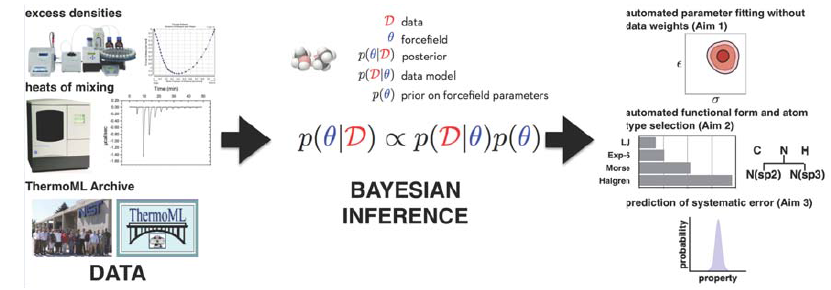
\includegraphics[width=1.0\textwidth]{Bayesian_inference_workflow}
  \caption{A schematic overview of the bayesian inference workflow where we derive parameters from experimental data}
 \end{figure}
  

\subsection{Methods $\left(1.5 pages \pm 0.5 pages\right)$}

\subsection{Progress $\left(1.5 pages \pm 0.5 pages\right)$}

\subsection{Research plan $\left(0.5 pages\right)$}

\bibliographystyle{IEEEtran}
\bibliography{report_outline}

\end{document}
